% !TeX root = ..\studio-operation-guide.tex
\section{Call Mute}

You can mute the microphone of the active audio device during an active
call so that the other party cannot hear you. Call mute applies to all
modes (Handset, Headset and Speakerphone).

\subsubsection{To mute a call:}

\begin{enumerate}
	\item Press	\scalerel*{
\includegraphics{images/yealink/btn-mute.png}}{B}
		during an active call.
	
		The LCD screen indicates that the call is now muted.
	
		\begin{figure}[h]
			\centering
			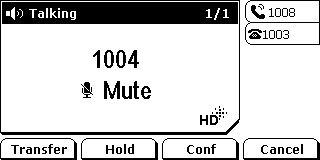
\includegraphics{images/yealink/screen-005.png}
		\end{figure}
\end{enumerate}

\subsubsection{To un-mute a call:}

\begin{enumerate}
	\item Press \scalerel*{
\includegraphics{images/yealink/btn-mute.png}}{B}
		again to un-mute the call.
\end{enumerate}
